\section{Evaluation Design and Audited Model Results}
\label{sec:evaluation}

The evaluation reports four kinds of output: agreement with filing-derived labels, performance against development labels, comparison with historical human ratings, and saved company scores. Final values come from the consolidated audit and recovered-result JSON files. Each comparison records the dataset, reference source, and unit of analysis.

\subsection{Data groups, evaluation measures, and uncertainty}

For principle classification, Top-1 agreement is the share of text segments whose highest-ranked principle matches the recorded label. Top-2 agreement is the share whose recorded label appears among the two highest-ranked principles. Top-2 gives an analyst a short candidate list. A higher Top-2 value does not mean better accuracy when only one answer is allowed.

Precision shows how reliable a predicted category is. If 100 text segments receive an environmental-principle prediction and 90 carry that reference label, precision is 90\%. Recall shows how much of a reference category is found. If 100 text segments carry the environmental label and the classifier finds 80, recall is 80\%. F1 balances precision and recall through the harmonic mean:
\begin{equation}
F1_k=\frac{2P_kR_k}{P_k+R_k},\qquad
\operatorname{MacroF1}=\frac{1}{9}\sum_{k=1}^{9}F1_k.
\label{eq:f1}
\end{equation}
Macro-F1 gives each principle equal weight, so the largest class cannot determine the entire score. Support means the number of reference examples for a principle. The references are weak labels. A result described as correct therefore means agreement with the recorded assignment, not an independent judgement of the text segment's meaning.

A 95\% confidence interval shows uncertainty in an estimate under the stated sampling method. For classification and mapping, the audit uses 2,000 bootstrap samples with seed 4206. Companies are sampled with replacement, and all text segments from a selected CIN are kept together. This CIN-cluster method accounts for text segments from the same company being related. Paired comparisons use the same sampled companies for both methods. These intervals describe variation within the available data; label errors and earlier exposure during model development remain outside that estimate. The 20-company score comparison uses 10,000 bootstrap samples of company-score pairs with seed 42. No detector intervals were calculated.

\subsection{Method comparisons and generalisation checks}
\label{sec:comparison_summary}

Before the detailed results, Table~\ref{tab:comparison_summary} gives a short overview of three comparisons. The first looks at how well the classifier agrees with the weak labels from each label source. The second tests the classifier on reporting concepts that were left out of training. The third sets the supervised BERT classifier against the zero-shot MPNet method. For each comparison, the table lists the text segments used and the training conditions. The three rows differ in data and in training, so the comparisons should be read separately and not as the result of changing a single component.

\begin{table}[tbp]
\centering\small
\caption{Three comparisons of Top-1 agreement with weak labels. The text segments and training conditions are listed for each row. Percentages from different rows describe different groups of text segments. Sections~\ref{sec:eval_sources}, \ref{sec:concept_diagnostics}, and~\ref{sec:eval_mapping} give intervals and further measures.}
\label{tab:comparison_summary}
\begin{tabularx}{\linewidth}{@{}L{2.6cm}L{2.5cm}L{3.1cm}Y@{}}
\toprule\textbf{Comparison} & \textbf{Evaluation population} & \textbf{Top-1 agreement} & \textbf{Interpretation}\\\midrule
Label source & B: 352; C: 5,364; notes: 485 text segments & B: 63.35\%; C: 95.15\%; notes: 90.72\% & Results for parts of the same 6,201-text-segment test group. The sources use different text and labelling rules.\\
Full-concept and excluded-concept training & Same 1,190 text segments from 174 companies & Full concept: 97.98\%; excluded concept: 87.31\% & The two training sets differ in concept coverage, number of training examples, and seed.\\
Zero-shot MPNet versus supervised BERT & Same 6,201 text segments from 175 companies & MPNet: 67.63\%; BERT: 93.00\% & The two methods have different access to labels. The BERT value reuses the classifier result.\\\bottomrule
\end{tabularx}
\end{table}

The reported comparisons use the final labelled split and the training conditions listed in the table. Domain adaptation is part of the final model's training sequence. No separate numerical gain is assigned to adaptation or data cleaning.

\subsection{Dataset size and results by label source}
\label{sec:eval_sources}

The final single-label dataset contains 42,409 dataset rows: 2,479 from explicit principle-axis facts, 36,513 from Section C mappings, and 3,417 from principle notes. The builder excludes 36,491 noisy facts and removes 2,640 groups with several labels. Fact rows and groups are different counting units. These exclusions cannot simply be added as final examples.

The Section B build starts with 41,898 narrative candidates. The content filter removes 16,684 candidates, leaving 25,214 clean entries. Removing 18 repeated same-label entries and 22,717 entries from groups with several labels produces 2,479 final dataset rows. These steps reconcile the current source counts. Table~\ref{tab:class_counts} lists the final dataset and test-set counts for each principle.

\begin{table}[tbp]
\centering\small
\caption{Final weak-label dataset by principle. The last column gives example counts in the company-separated test set.}
\label{tab:class_counts}
\begin{tabularx}{\linewidth}{@{}Yr r@{}}
\toprule\textbf{Principle} & \textbf{Dataset rows} & \textbf{Test rows}\\\midrule
P1: Ethics and governance & 5,015 & 773\\
P2: Sustainable goods and services & 5,566 & 808\\
P3: Employee and worker wellbeing & 11,835 & 1,715\\
P4: Stakeholder interests & 3,128 & 469\\
P5: Human rights & 3,095 & 449\\
P6: Environmental responsibility & 5,749 & 823\\
P7: Public policy advocacy & 543 & 69\\
P8: Inclusive growth & 2,475 & 368\\
P9: Consumer responsibility & 5,003 & 727\\\midrule
\textbf{Total} & \textbf{42,409} & \textbf{6,201}\\\bottomrule
\end{tabularx}
\end{table}

\begin{table}[tbp]
\centering\small
\caption{Recovered classifier results by label source on the same test set. A company can supply several sources, so the company counts overlap. Top-1 intervals are calculated by resampling companies.}
\label{tab:source}
\begin{tabularx}{\linewidth}{@{}Yrrrrl@{}}
\toprule\textbf{Source} & \textbf{Text segments} & \textbf{CINs} & \textbf{Top-1} & \textbf{Top-2} & \textbf{Top-1 95\% CI}\\\midrule
Section B: explicit axis & 352 & 71 & 63.35\% & 80.40\% & 56.55--69.67\%\\
Section C: concept map & 5,364 & 174 & 95.15\% & 99.01\% & 94.41--95.92\%\\
Principle notes & 485 & 103 & 90.72\% & 95.46\% & 86.55--94.09\%\\\bottomrule
\end{tabularx}
\end{table}

Table~\ref{tab:source} reports agreement of 63.35\% for explicit-axis text segments and 95.15\% for concept-mapped text segments. Section C supplies 86.1\% of the full labelled dataset and 5,364 of the 6,201 test rows. The overall value therefore reflects the source mix. Section B contains the examples retained by the single-label filtering procedure. Figure~\ref{fig:source} presents the three sources together, and the excluded-concept tests provide a second view of performance across reporting questions.

\begin{figure}[tbp]
\centering
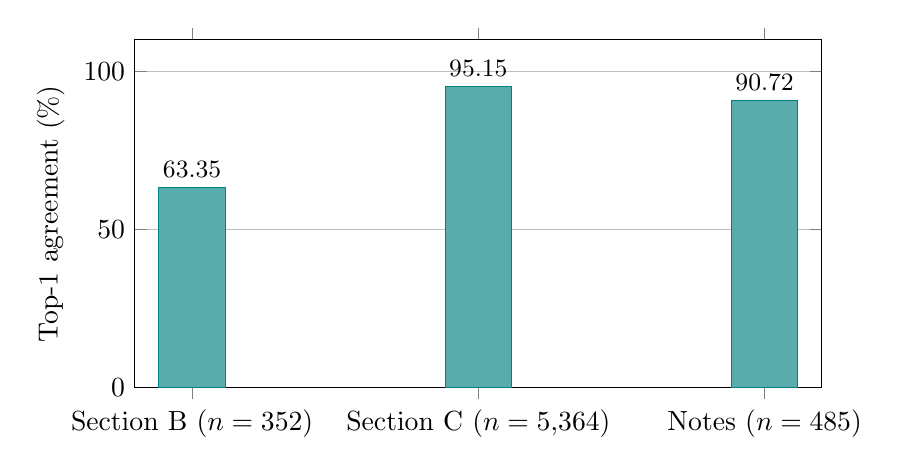
\begin{tikzpicture}
\begin{axis}[width=0.85\linewidth,height=6cm,ybar,bar width=24pt,
  ylabel={Top-1 agreement (\%)},ymin=0,ymax=110,
  symbolic x coords={B,C,Notes},xtick=data,
  xticklabels={Section B ($n=352$),Section C ($n=5{,}364$),Notes ($n=485$)},
  ymajorgrids=true,nodes near coords,nodes near coords style={font=\small},
  point meta=explicit symbolic]
\addplot[fill=teal!65,draw=teal] coordinates {(B,63.35) [63.35] (C,95.15) [95.15] (Notes,90.72) [90.72]};
\end{axis}
\end{tikzpicture}
\caption{Principle-label agreement by source. The bars compare explicitly tagged passages, concept-mapped passages, and principle notes using the filing-derived reference labels. Table~\ref{tab:source} gives confidence intervals calculated by resampling companies.}
\label{fig:source}
\end{figure}


\subsection{Recovered classifier performance and training history}
\label{sec:training_history}

The recovered seed-99 model matches 5,767 of 6,201 reference labels. Top-1 agreement is 93.00\% (95\% CI: 92.04--93.89\%). The reference label appears among the two highest predictions for 6,057 examples, giving 97.68\% Top-2 agreement (95\% CI: 97.10--98.21\%). Macro-F1 is 0.9158 (95\% CI: 0.9036--0.9277). The text-overlap check identifies 50 exact train/test matches across different companies, or 0.81\% of test rows. The supervised split has zero CIN overlap.

Figure~\ref{fig:training} shows the five recorded epochs for seed 99. Validation macro-F1 rises from 0.9048 at epoch 1 to 0.9194 at epoch 4, then reaches 0.9189 at epoch 5. Validation loss rises over the same period. F1 describes category decisions, while loss also considers prediction confidence. The recorded selection criterion chooses epoch 4 by validation macro-F1.

\begin{figure}[tbp]
\centering
\begin{subfigure}{0.48\linewidth}
\centering
\begin{tikzpicture}
\begin{axis}[width=\linewidth,height=5.4cm,xlabel={Completed epoch},ylabel={Validation macro-F1},
  xmin=0.7,xmax=5.3,ymin=0.895,ymax=0.925,xtick={1,2,3,4,5},ymajorgrids=true,
  scaled y ticks=false,yticklabel style={/pgf/number format/fixed,/pgf/number format/precision=3}]
\addplot[teal,thick,mark=*] coordinates {(1,0.904818)(2,0.907187)(3,0.913640)(4,0.919368)(5,0.918854)};
\addplot[warm,only marks,mark=*,mark size=3.5pt] coordinates {(4,0.919368)};
\end{axis}
\end{tikzpicture}
\caption{Category agreement is highest at epoch 4.}
\end{subfigure}\hfill
\begin{subfigure}{0.48\linewidth}
\centering
\begin{tikzpicture}
\begin{axis}[width=\linewidth,height=5.4cm,xlabel={Completed epoch},ylabel={Validation loss},
  xmin=0.7,xmax=5.3,ymin=0.25,ymax=0.50,xtick={1,2,3,4,5},ymajorgrids=true]
\addplot[ink,thick,mark=square*] coordinates {(1,0.310062)(2,0.360093)(3,0.401145)(4,0.447556)(5,0.468024)};
\end{axis}
\end{tikzpicture}
\caption{Loss records changes in prediction confidence.}
\end{subfigure}
\caption{Five recorded training epochs for seed 99. The marked point identifies checkpoint 7,460, selected by validation macro-F1. The two panels present category agreement and probability-based loss, showing the recorded basis for checkpoint selection.}
\label{fig:training}
\end{figure}


Table~\ref{tab:per_principle} groups performance by principle; Table~\ref{tab:source} groups performance by label source. Each principle row shows prediction reliability, reference-category coverage, and the balance between both. P7 has only 69 test examples, so the P7 estimate needs extra care. Figure~\ref{fig:per_principle} summarises F1, while the table also gives precision, recall, and example counts.

\begin{table}[tbp]
\centering\small
\caption{Results for nine principles on 6,201 text segments. Precision shows how often a predicted principle matches the reference. Recall shows how much of the reference category is found. F1 balances both.}
\label{tab:per_principle}
\begin{tabularx}{\linewidth}{@{}Yrrrr@{}}
\toprule\textbf{Principle} & \textbf{Support} & \textbf{Precision} & \textbf{Recall} & \textbf{F1}\\\midrule
P1: Ethics and governance & 773 & 0.9592 & 0.9431 & 0.9511 \\
P2: Sustainable goods and services & 808 & 0.9154 & 0.8837 & 0.8992 \\
P3: Employee and worker wellbeing & 1,715 & 0.9533 & 0.9644 & 0.9588 \\
P4: Stakeholder interests & 469 & 0.9611 & 0.9488 & 0.9549 \\
P5: Human rights & 449 & 0.9009 & 0.8508 & 0.8751 \\
P6: Environmental responsibility & 823 & 0.8943 & 0.9356 & 0.9145 \\
P7: Public policy advocacy & 69 & 0.8551 & 0.8551 & 0.8551 \\
P8: Inclusive growth & 368 & 0.8921 & 0.9212 & 0.9064 \\
P9: Consumer responsibility & 727 & 0.9259 & 0.9285 & 0.9272 \\
\midrule
Macro average & 6,201 & 0.9175 & 0.9146 & 0.9158\\\bottomrule
\end{tabularx}
\end{table}

\begin{figure}[tbp]
\centering
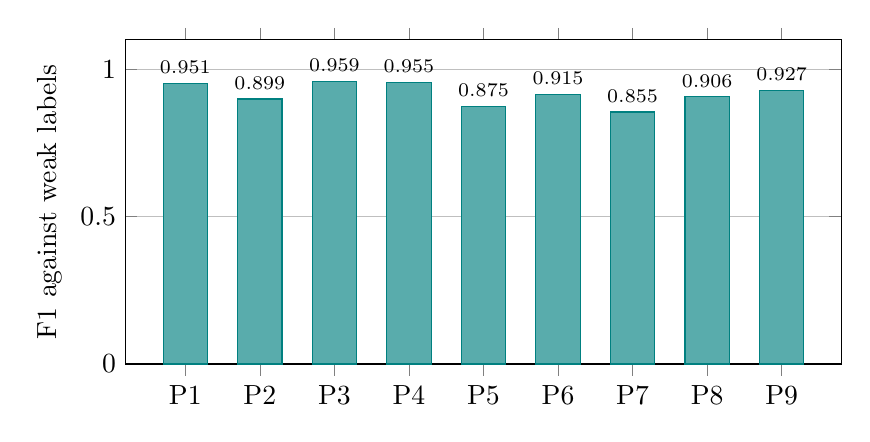
\begin{tikzpicture}
\begin{axis}[width=0.88\linewidth,height=5.7cm,ybar,bar width=16pt,ymin=0,ymax=1.10,
  ylabel={F1 against weak labels},symbolic x coords={P1,P2,P3,P4,P5,P6,P7,P8,P9},xtick=data,
  ymajorgrids=true,nodes near coords,nodes near coords style={font=\scriptsize,/pgf/number format/fixed,/pgf/number format/precision=3}]
\addplot[fill=teal!65,draw=teal] coordinates {(P1,0.9511)(P2,0.8992)(P3,0.9588)(P4,0.9549)(P5,0.8751)(P6,0.9145)(P7,0.8551)(P8,0.9064)(P9,0.9272)};
\end{axis}
\end{tikzpicture}
\caption{F1 by principle for the recovered classifier. A higher bar means a better balance of precision and recall against the recorded weak labels. P7 has 69 test examples, compared with 1,715 for P3. Table~\ref{tab:per_principle} gives all example counts and measures.}
\label{fig:per_principle}
\end{figure}


\subsection{Tests on excluded concepts and multiple labels}
\label{sec:concept_diagnostics}

Two kinds of separation are tested. The first, separating companies, asks whether the model can classify text segments from a company excluded from supervised training. The second, separating concepts, asks whether the model can classify text segments that answer reporting questions left out of labelled training. For the concept test, 17 Section C concepts were excluded, and 1,190 dataset rows were evaluated. On these same dataset rows, the full-concept model reaches 97.98\% Top-1 agreement, while the excluded-concept model reaches 87.31\%. The paired difference is $-10.67$ percentage points (95\% CI: $-12.36$ to $-8.96$). Before re-evaluation, both checkpoints passed strict parameter-name recovery.

The two models were not trained under identical conditions. The full-concept model uses seed 99. The excluded-concept model uses seed 42 and fewer training examples. The paired interval therefore describes the difference on shared test dataset rows under these conditions, and the gap reflects concept coverage, the number of training examples, and the seed together, not concept exclusion alone.

The excluded-concept training was repeated in three runs. The mean Top-1 agreement across the three runs is 81.64\%, with a sample standard deviation of 4.92 percentage points. The mean Top-2 agreement is 95.34\% (standard deviation 1.31 percentage points), and the mean macro-F1 is 0.6752 (standard deviation 0.0170). Figure~\ref{fig:concept} shows each run and the corresponding test size. The standard deviations measure how much the three runs differ from one another. All three runs reuse the original test-company group, and concept exclusion applies to labelled training only. The adaptation-corpus membership of the earlier model is described in Section~\ref{sec:classifier}.

\begin{figure}[tbp]
\centering
\begin{tikzpicture}
\begin{axis}[width=0.90\linewidth,height=6.2cm,ybar,bar width=17pt,ymin=0,ymax=112,
  ylabel={Top-1 agreement (\%)},symbolic x coords={H42,H17,H73},xtick=data,
  xticklabels={Test 42 ($n=1{,}190$),Test 17 ($n=1{,}167$),Test 73 ($n=1{,}169$)},
  ymajorgrids=true,legend style={at={(0.5,1.04)},anchor=south,legend columns=2},
  nodes near coords,nodes near coords style={font=\scriptsize,/pgf/number format/fixed,/pgf/number format/precision=2}]
\addplot[fill=ink!35,draw=ink] coordinates {(H42,97.98)(H17,96.06)(H73,97.18)};
\addlegendentry{Full-concept model}
\addplot[fill=teal!65,draw=teal] coordinates {(H42,87.31)(H17,79.18)(H73,78.44)};
\addlegendentry{Excluded-concept model}
\end{axis}
\end{tikzpicture}
\caption{Full-concept and excluded-concept training on three shared test groups. The tests contain 174, 173, and 174 companies from the original split. Excluded-concept mean agreement is 81.64\%, with sample standard deviation 4.92 percentage points across runs. Training examples and seeds are described in Section~\ref{sec:concept_diagnostics}; the standard deviation summarises variation across these runs.}
\label{fig:concept}
\end{figure}


\subsection{Frozen text-vagueness results}

Table~\ref{tab:detector} lists how the fixed detector performed on two separate groups of examples. The first group, Batches 1 and 2, has 80 earlier development examples. The reference label marks 37 text segments as vague, and the detector raises 41 flags. Only 29 of these flags agree with the reference. Out of 41 flags, 29 were right, which is a precision of 0.7073. Out of 37 vague examples, 29 were found, which is a recall of 0.7838. Accuracy counts every decision, flagged or not. Here 60 of the 80 decisions match the reference, so accuracy is 0.7500. F1, the balance between precision and recall, is 0.7436.

Batch 3 forms the second group. The 70 examples of this batch were labelled by AI, and not by the earlier development process. The detector flags 35 text segments, and 21 of the flags match the AI label. The AI label marks 26 text segments as vague, so the detector found 21 of 26. F1 for this group is 0.6885. Figure~\ref{fig:detector} puts precision, recall, and F1 of this group beside the 80-example group. The two groups differ in text segments and in the source of the reference, so the results are not merged.

\begin{table}[tbp]
\centering\small
\caption{Fixed text-vagueness detector on two label groups. The first row uses 80 development examples, and the second uses 70 AI-labelled examples. Reference conditions are stated in the evaluation text.}
\label{tab:detector}
\begin{tabularx}{\linewidth}{@{}Yrrrrr@{}}
\toprule\textbf{Reference labels} & \textbf{N} & \textbf{Accuracy} & \textbf{Precision} & \textbf{Recall} & \textbf{F1}\\\midrule
Historical development labels & 80 & 0.7500 & 0.7073 & 0.7838 & 0.7436\\
AI annotations & 70 & 0.7286 & 0.6000 & 0.8077 & 0.6885\\\bottomrule
\end{tabularx}
\end{table}

\begin{figure}[tbp]
\centering
\begin{tikzpicture}
\begin{axis}[width=0.85\linewidth,height=6cm,ybar,bar width=17pt,ymin=0,ymax=1.12,
  ylabel={Decision measure},symbolic x coords={Precision,Recall,F1},xtick=data,
  ymajorgrids=true,legend style={at={(0.5,1.03)},anchor=south,legend columns=1},
  nodes near coords,nodes near coords style={font=\scriptsize,/pgf/number format/fixed,/pgf/number format/precision=3}]
\addplot[fill=ink!35,draw=ink] coordinates {(Precision,0.7073)(Recall,0.7838)(F1,0.7436)};
\addlegendentry{Development reference ($n=80$)}
\addplot[fill=teal!65,draw=teal] coordinates {(Precision,0.6000)(Recall,0.8077)(F1,0.6885)};
\addlegendentry{AI reference ($n=70$, exploratory)}
\end{axis}
\end{tikzpicture}
\caption{Precision, recall, and F1 for the fixed language detector. The first group contains 80 development examples; the second contains 70 AI-labelled examples. Precision describes how often a flag matches the reference, recall describes how many reference-vague passages are found, and F1 balances both. These measures cover the language branch.}
\label{fig:detector}
\end{figure}


\subsection{Supervised transfer versus zero-shot mapping}
\label{sec:eval_mapping}

The same 6,201 test text segments were ranked by two methods. The first is the MPNet definition-plus-anchor method, which has no training on the labelled data. The method reaches a Top-1 agreement of 67.63\% and a Top-2 agreement of 83.34\%. The second is the recovered supervised classifier, which was trained on the labels and reaches 93.00\% and 97.68\%. The confidence intervals for both methods are given in Table~\ref{tab:mapping}. The paired Top-1 difference shows the supervised classifier agreeing with the recorded principle label more often, by $+25.37$ percentage points (95\% CI: $+24.02$ to $+26.71$). The size of this gap should be read with care. Two things differ between the methods, the model representation and the access to labelled training, so the gap cannot be credited to the representation alone. Both results measure agreement with the recorded principle label.

\begin{table}[tbp]
\centering\small
\caption{Principle mapping on the same company-separated test rows. Intervals resample companies. The supervised row reuses the classifier result and is not a second independent test.}
\label{tab:mapping}
\begin{tabularx}{\linewidth}{@{}Yrrl@{}}
\toprule\textbf{Method} & \textbf{Top-1} & \textbf{Top-2} & \textbf{Macro-F1}\\\midrule
MPNet zero-shot hybrid & 67.63\% & 83.34\% & 0.6405\\
\quad 95\% interval & 66.45--68.93\% & 82.31--84.38\% & 0.6248--0.6567\\
Recovered supervised transfer & 93.00\% & 97.68\% & 0.9158\\
\quad 95\% interval & 92.04--93.89\% & 97.10--98.21\% & 0.9036--0.9277\\\bottomrule
\end{tabularx}
\end{table}

The supervised row reuses the classifier evaluation from the same company-separated test set. Both methods are compared against the filing-derived reference labels defined in Section~\ref{sec:labels}. The result is reported once as an underlying model evaluation and reused for the mapping application.

\subsection{Transparency Score compared with historical human ratings}

The historical human-rating group contains 20 companies. Pearson correlation measures how automated and human scores vary together: $r=0.6314$ (95\% CI: 0.2683--0.8519; $p=0.0028$). Spearman correlation compares score ranks: $\rho=0.6285$ (95\% CI: 0.2321--0.8540). Mean absolute error is 12.16 points, and root mean squared error, which gives larger errors more weight, is 15.19 points. The audit reports $r^2=0.3986$. This squared correlation describes association; no separate predictive regression was fitted for this result.

The historical comparison uses 20 company ratings from one documented source. The saved file contains both ratings and automated scores; rater blinding is not documented. The original Zensar text packet includes a URL-related extraction issue, and Geojit's business model differs from manufacturing-oriented reporting items. Both companies remain in the full group. The analysis uses the original ratings and fixed score formula, with all 20 cases retained; synthetic ratings and AI assessments are kept separate.

\subsection{Checking the API connection}

The audit records a successful principle-mapping API request for 360 ONE WAM LIMITED on 19 October 2026. The response identifies the recovered seed-99 classifier and checkpoint path. The returned 89.17\% summary is the average model probability for that filing. This request verifies model loading for one company.

\FloatBarrier